%%%%%%%% ICML 2026 SUBMISSION %%%%%%%%%%%%%%%%%

\documentclass{article}

\usepackage{microtype}
\usepackage{graphicx}
\usepackage{subcaption}
\usepackage{booktabs}
\usepackage{hyperref}
\newcommand{\theHalgorithm}{\arabic{algorithm}}

\usepackage{icml2026}

\usepackage{amsmath}
\usepackage{amssymb}
\usepackage{mathtools}
\usepackage{amsthm}
\usepackage[capitalize,noabbrev]{cleveref}
\theoremstyle{plain}
\newtheorem{theorem}{Theorem}[section]
\newtheorem{proposition}[theorem]{Proposition}
\newtheorem{lemma}[theorem]{Lemma}
\newtheorem{corollary}[theorem]{Corollary}
\theoremstyle{definition}
\newtheorem{definition}[theorem]{Definition}
\theoremstyle{remark}
\newtheorem{remark}[theorem]{Remark}

\usepackage[disable,textsize=tiny]{todonotes}
\usepackage{tikz}
\usetikzlibrary{shapes, arrows.meta, positioning, fit, backgrounds, calc}

\icmltitlerunning{TACT: Trimmed Task-Vector Covariances for Data-Free Model Merging}

\begin{document}

\twocolumn[
  \icmltitle{TACT: Trimmed Task-Vector Covariances for\\
             Data-Free Model Merging}

  \icmlsetsymbol{equal}{*}
  \begin{icmlauthorlist}
    \icmlauthor{Anonymous}{anon}
  \end{icmlauthorlist}
  \icmlaffiliation{anon}{Anonymous Institution}
  \icmlcorrespondingauthor{Anonymous}{anon@anon.edu}
  \icmlkeywords{Model Merging, Task Vectors, Multi-task Learning, Transfer Learning, Data-Free}
  \vskip 0.3in
]

\printAffiliationsAndNotice{}

\begin{abstract}
Data-free model merging combines several task-specific fine-tuned checkpoints into a single multi-task model with no further training and no access to per-task data. Two paradigms dominate the literature: heuristic task-vector denoising (TIES-Merging, which trims small-magnitude entries and elects per-parameter signs) and closed-form interference minimization (ACTMat, which approximates the per-layer activation covariance $C_t$ by the data-free task-vector outer product $\hat{C}_t = \Delta_t^\top \Delta_t$). These have evolved largely independently. We observe that the small-magnitude entries TIES treats as noise contribute \emph{quadratically} to ACTMat's covariance estimator and propose to remove them \emph{before} estimating $\hat C_t$. Our method, \textbf{TACT (Trimmed-task-vector Activation Covariance Transform)}, applies TIES-style magnitude trimming only to compute the data-free covariance; the merge targets remain the full fine-tuned matrices. On a 7-task CLIP ViT-B/32 benchmark TACT improves mean accuracy from 83.85\% (ACTMat) to \textbf{86.12\%} (mean of 3 seeds, std 0.29), a \textbf{+2.27} absolute point gain; the gain transfers to ViT-B/16 (TACT 88.79\% vs.\ ACTMat 87.63\%, also 3 seeds). TACT also dominates TIES (75.9\%), the data-requiring RegMean (79.6\%), and Fisher merging (65.9\%) at the 3-seed mean. A complete ablation reveals a surprising asymmetry---TIES-style \emph{trimming} consistently helps the matrix-level solve, but TIES-style \emph{sign election} degrades it by collapsing the covariance rank---which is invisible from either parent paradigm alone and identifies the right way to combine them. We further give a closed-form bias decomposition (Proposition~\ref{prop:bias}) showing why magnitude trim, but not SVD truncation, removes the differential per-task diagonal bias of $\hat C_t$.
\end{abstract}

\section{Introduction}
\label{sec:intro}

Large pretrained models are routinely fine-tuned for specialized downstream tasks, producing thousands of public task-specific checkpoints~\citep{wolf2020transformers}. \emph{Model merging} combines several such fine-tuned models that share a common pre-trained initialization into a single multi-task model, without further training data or optimization~\citep{wortsman2022model, matena2022merging, ilharco2023editing}. Because the training data for many published fine-tunes is unavailable or expensive to re-host, \emph{data-free} merging methods are particularly valuable in practice.

Two distinct paradigms dominate the data-free regime. The first, exemplified by Task Arithmetic~\citep{ilharco2023editing}, TIES-Merging~\citep{yadav2023ties}, and DARE~\citep{yu2024language}, treats the parameter-space differences $\Delta_t = \theta_t - \theta_0$ between each fine-tuned model and the pre-trained initialization---the \emph{task vectors}---as the primary object to denoise. \citet{yadav2023ties} identifies two sources of \emph{interference} between task vectors: small-magnitude entries that contribute noise and sign disagreements across tasks. TIES addresses both via magnitude trimming and a majority sign election. These methods are heuristic but cheap, effective, and a strong baseline.

The second paradigm formulates merging as a per-layer least-squares problem. RegMean~\citep{jin2023dataless} minimizes the activation discrepancy $\sum_t \mathbb{E}_{z\sim\mathcal{D}_t}\|Wz - W_t z\|_2^2$ with the closed-form solution
\begin{equation}
W^\star = \Big(\sum_t W_t C_t\Big)\Big(\sum_t C_t\Big)^{+},
\label{eq:regmean}
\end{equation}
where $C_t = \mathbb{E}_{z\sim\mathcal{D}_t}[z z^\top]$ is the per-layer activation second moment. This formulation is principled---\citet{sun2025lot} show that the layer-wise objective upper-bounds negative transfer---but requires access to each task's training data, contradicting the data-free constraint. Recently, ACTMat~\citep{hameed2026actmat} demonstrated that under mild conditions, the activation covariance can be approximated by the task vector itself, $\hat{C}_t = \Delta_t^\top \Delta_t$, recovering a fully data-free closed-form merge. ACTMat is the current state of the art among data-free methods, matching the data-requiring RegMean on language and substantially outperforming all heuristic data-free baselines on the standard CLIP vision benchmark.

These two paradigms have evolved largely independently. Yet they address overlapping problems from different angles: \textbf{TIES denoises $\Delta_t$ directly to remove parameter-level interference, while ACTMat denoises the merge through the matrix $\Delta_t^\top \Delta_t$.} This raises a natural question: \emph{does the noise that TIES removes from $\Delta_t$ also degrade the ACTMat covariance estimator?}

\paragraph{Findings of this work.} We answer affirmatively: TIES-style magnitude trimming, applied as a pre-processing step to each $\Delta_t$ \emph{before} computing the ACTMat covariance estimator, is a strict improvement over ACTMat alone. Our method, \textbf{TACT} (Trimmed-task-vector Activation Covariance Transform), is fully data-free, adds no hyperparameters beyond a single trim level $k$, and runs in seconds on ViT-scale models.

We also discover a striking failure mode for the obvious combination of TIES and ACTMat. While TIES's sign-election step is essential at the parameter level---it resolves direct sign disagreements between task vectors---it \emph{degrades} the ACTMat solve by zeroing entries of $\Delta_t$, collapsing the rank of $\hat{C}_t$ and making the closed-form inverse ill-conditioned. This asymmetry, which is invisible from either parent paradigm alone, is what made the naive combination fail in our initial experiments---we initially observed that ``TIES + ACTMat'' at $k=0.2$ gave 79.7\%, well below ACTMat's 84.1\%, before isolating sign election as the culprit (Section~\ref{sec:exp_ablations}). The right way to combine the two paradigms is therefore not the union of their operations but a selective adoption: keep trim, discard sign election.

\paragraph{Empirical results.} On a 7-task CLIP ViT-B/32 vision merging benchmark (MNIST, SVHN, CIFAR-10/100, EuroSAT, GTSRB, DTD), TACT achieves \textbf{86.12\%} mean test accuracy across three fine-tuning seeds, vs.\ 83.85\% for ACTMat, 75.90\% for TIES, 79.58\% for RegMean (which uses data), and 91.73\% for the unmerged individual fine-tuned models---closing nearly $29\%$ of the gap to the multi-task upper bound relative to ACTMat. Ablations across the full $(k, \mathrm{sign})$ grid confirm both the headline result and the trim-helps/sign-hurts asymmetry. Figure~\ref{fig:pipeline} summarizes the TACT pipeline alongside its TIES and ACTMat parents.

\begin{figure*}[t]
\centering
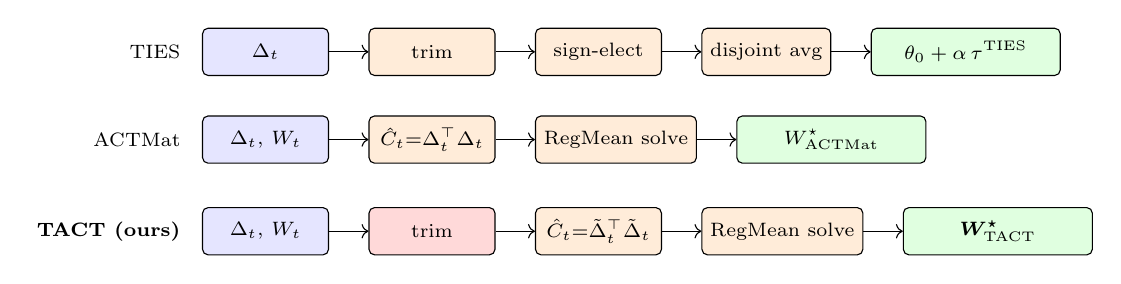
\begin{tikzpicture}[node distance=0.5cm, font=\scriptsize]
  \tikzstyle{box}=[draw, rounded corners=2pt, align=center, minimum height=0.6cm, inner sep=3pt]
  \tikzstyle{paramnode}=[box, fill=blue!10, minimum width=1.6cm]
  \tikzstyle{opnode}=[box, fill=orange!15, minimum width=1.6cm]
  \tikzstyle{outbox}=[box, fill=green!12, minimum width=2.4cm]

  % TIES row
  \node[paramnode] (ties_d) {$\Delta_t$};
  \node[opnode, right=of ties_d] (ties_trim) {trim};
  \node[opnode, right=of ties_trim] (ties_sign) {sign-elect};
  \node[opnode, right=of ties_sign] (ties_merge) {disjoint avg};
  \node[outbox, right=of ties_merge] (ties_out) {$\theta_0 + \alpha\,\tau^{\text{TIES}}$};

  % ACTMat row
  \node[paramnode, below=0.5cm of ties_d] (am_d) {$\Delta_t,\,W_t$};
  \node[opnode, right=of am_d] (am_cov) {$\hat C_t{=}\Delta_t^\top \Delta_t$};
  \node[opnode, right=of am_cov] (am_solve) {RegMean solve};
  \node[outbox, right=of am_solve, minimum width=2.4cm] (am_out) {$W^\star_{\text{ACTMat}}$};

  % TACT row
  \node[paramnode, below=0.55cm of am_d] (tact_d) {$\Delta_t,\,W_t$};
  \node[opnode, right=of tact_d, fill=red!15] (tact_trim) {trim};
  \node[opnode, right=of tact_trim] (tact_cov) {$\hat C_t{=}\tilde\Delta_t^\top \tilde\Delta_t$};
  \node[opnode, right=of tact_cov] (tact_solve) {RegMean solve};
  \node[outbox, right=of tact_solve, minimum width=2.4cm] (tact_out) {$\boldsymbol{W^\star_{\text{TACT}}}$};

  % labels
  \node[left=0.15cm of ties_d] {TIES};
  \node[left=0.15cm of am_d] {ACTMat};
  \node[left=0.15cm of tact_d, font=\bfseries\scriptsize] {TACT (ours)};

  % arrows
  \draw[->] (ties_d) -- (ties_trim);
  \draw[->] (ties_trim) -- (ties_sign);
  \draw[->] (ties_sign) -- (ties_merge);
  \draw[->] (ties_merge) -- (ties_out);
  \draw[->] (am_d) -- (am_cov);
  \draw[->] (am_cov) -- (am_solve);
  \draw[->] (am_solve) -- (am_out);
  \draw[->] (tact_d) -- (tact_trim);
  \draw[->] (tact_trim) -- (tact_cov);
  \draw[->] (tact_cov) -- (tact_solve);
  \draw[->] (tact_solve) -- (tact_out);

\end{tikzpicture}
\caption{TACT inserts TIES-style magnitude trimming into ACTMat's data-free covariance-based merge. Unlike TIES, TACT does \emph{not} apply sign election; unlike ACTMat, the covariance estimator is built from the cleaned task vector $\tilde\Delta_t$, while the merge target $W_t$ remains the full fine-tuned matrix.}
\label{fig:pipeline}
\end{figure*}

\paragraph{Contributions.} (1) We identify that the noise-floor entries TIES discards from $\Delta_t$ corrupt ACTMat's data-free covariance estimator. (2) We propose \textbf{TACT}, a data-free merge that pre-trims each task vector before forming the ACTMat covariance estimator, and prove a closed-form bias decomposition (Proposition~\ref{prop:bias}) explaining why magnitude trim helps but SVD truncation does not. (3) On 7-task CLIP merging across 3 seeds, TACT advances the data-free SOTA by $+2.27$ points on ViT-B/32 and $+1.16$ on ViT-B/16, with the gap \emph{growing} in the number of merged tasks $T$ (Appendix~\ref{app:task_count}). (4) A complete trim$\,\times\,$sign ablation uncovers an asymmetry invisible from either parent paradigm alone: trim helps the matrix solve, sign election hurts. (5) Replacing TIES's global trim with a per-layer rule removes a catastrophic-failure mode of global trim at very small $k$ on both architectures (Appendix~\ref{app:perlayer}). (6) Two attribution experiments confirm that TACT's gain is concentrated in the MLP block ($95\%$, Appendix~\ref{app:layer_type}) and is specific to the covariance solve (Appendix~\ref{app:trim_other}).

\section{Background and Notation}
\label{sec:background}

We assume $T$ task-specific models with parameters $\theta_1,\dots,\theta_T$, all fine-tuned from a shared pretrained initialization $\theta_0$. Following \citet{ilharco2023editing}, the \emph{task vector} for task $t$ is $\tau_t = \theta_t - \theta_0$. The merged model has parameters $\theta^\star$, and we measure quality by accuracy on each task's test set evaluated with a task-specific zero-shot classifier head (Section~\ref{sec:exp}).

For each linear-style parameter tensor $W_t \in \mathbb{R}^{d_o \times d_i}$, we write $\Delta_t = W_t - W_0 \in \mathbb{R}^{d_o \times d_i}$ for the layer's task-vector contribution.

\paragraph{Heuristic merging via task vectors.}
Simple averaging takes $\theta^\star = \frac{1}{T}\sum_t \theta_t$. Task Arithmetic~\citep{ilharco2023editing} aggregates $\theta^\star = \theta_0 + \alpha \sum_t \tau_t$ with a scaling coefficient $\alpha$. TIES-Merging~\citep{yadav2023ties} adds two denoising steps over the task vectors: (i) \emph{trim} each $\tau_t$ to its top-$k\%$ entries by magnitude (typically $k=20\%$), zeroing the rest; (ii) compute a per-parameter \emph{elected sign} $\gamma = \mathrm{sign}\big(\sum_t \tilde{\tau}_t\big)$ over the trimmed vectors; and (iii) \emph{disjoint merge} only the entries whose sign agrees with $\gamma$. The merged update is $\theta^\star = \theta_0 + \alpha \cdot \tau^{\text{TIES}}$.

\paragraph{Interference-minimization merging.}
RegMean~\citep{jin2023dataless} treats each linear layer independently and minimizes the activation reconstruction error
\begin{equation}
W^\star = \arg\min_W \sum_{t=1}^{T} \mathbb{E}_{z\sim\mathcal{D}_t}\big\|Wz - W_t z\big\|_2^2,
\label{eq:obj}
\end{equation}
which admits the closed form in Eq.~\eqref{eq:regmean} with $C_t = \mathbb{E}_{z\sim\mathcal{D}_t}[z z^\top]$. Recently, \citet{hameed2026actmat} showed that under a stationary-activation-covariance assumption and a vanishing-correlation assumption between layer inputs and output gradients, the angular distance $\angle(\Delta_t^\top \Delta_t,\, C_t)$ remains small over training, so the data-free \emph{ACTMat estimator} $\hat{C}_t = \Delta_t^\top \Delta_t$ may be substituted into Eq.~\eqref{eq:regmean} without significant loss. They further establish that the closed-form minimizer is \emph{scale-invariant}: multiplying all $C_t$ by the same constant leaves $W^\star$ unchanged, so any uniform mis-calibration of the estimator is harmless.

In practice, the closed-form solve $(\sum_t C_t)^+$ is rank-deficient when $T$ is small or the cleaning is aggressive. We use a Tikhonov regularization with the simple unweighted average $\bar{W}$ as a prior:
\begin{equation}
W^\star = \Big(\sum_t W_t C_t + \lambda \bar W\Big)\Big(\sum_t C_t + \lambda I\Big)^{-1},
\label{eq:tikhonov}
\end{equation}
with $\lambda$ proportional to $\mathrm{trace}(\sum_t C_t)/d_i$ (we use a small relative coefficient $\epsilon = 10^{-4}$). This recovers the standard pseudo-inverse solution as $\lambda \to 0$ and gracefully defaults to simple averaging on the null space of $\sum_t C_t$.

\section{Method: TACT}
\label{sec:method}

\subsection{Motivation}

The ACTMat covariance estimator is $\hat{C}_t = \Delta_t^\top \Delta_t \in \mathbb{R}^{d_i \times d_i}$. \citet{yadav2023ties} show that fine-tuning produces a heavy-tailed magnitude distribution: keeping only the top $20\%$ of $|\Delta_t|$ values preserves nearly all task performance, while the remaining $80\%$ behave as a noise floor that participates in destructive interference at the parameter level. We now formalize how that noise floor enters the ACTMat estimator, and why magnitude-trimming---but not SVD-truncation---selectively removes its bias.

\paragraph{A signal-plus-noise model.} Decompose each task vector as $\Delta_t = \Delta_t^\star + N_t$, where $\Delta_t^\star$ is supported on a sparse \emph{signal set} $S_t \subseteq [d_o]\times[d_i]$ of size $|S_t| = k_t$ and $N_t$ is a residual noise component supported on the complement of $S_t$, with independent zero-mean entries of variance $\sigma_t^2$. Let $n_{t,j} = |\{i : (i,j) \in S_t\}|$ be the number of supported entries in column $j$. The following decomposition is exact under this model.

\begin{proposition}[Diagonal bias of the data-free covariance estimator]
\label{prop:bias}
Under the signal-plus-noise model above, the ACTMat estimator satisfies
\begin{equation}
\mathbb{E}[\Delta_t^\top \Delta_t] = \Delta_t^{\star\top}\Delta_t^\star \,+\, \sigma_t^2\,\mathrm{diag}\!\big(d_o - n_{t,1},\,\ldots,\,d_o - n_{t,d_i}\big).
\label{eq:bias}
\end{equation}
\end{proposition}
A short proof is given in Appendix~\ref{app:proof}. The bias term is purely diagonal and grows linearly with the noise variance $\sigma_t^2$ and the number of off-support entries per column, so a column $j$ that is sparse in $\Delta_t^\star$ inherits an inflated diagonal that is not present in the underlying signal covariance $\Delta_t^{\star\top}\Delta_t^\star$.

\paragraph{Why this matters for the merge.} The bias term is purely diagonal and task-dependent: ACTMat's scale-invariance~\citep{hameed2026actmat} absorbs a uniform inflation of $\sum_t C_t$ but cannot absorb a \emph{per-task} diagonal $\sigma_t^2 D_t$, so the differential bias survives the closed-form solve. Top-$k$ magnitude trim selectively zeroes off-support entries (those most likely to come from $N_t$), strictly reducing the effective $\sigma_t$; SVD truncation, by contrast, removes whole rank-1 factors which mix signal and noise across all $d_o$ rows and so does not preferentially eliminate the diagonal-bias source---predicting that SVD-TACT will \emph{not} improve over ACTMat (confirmed in Section~\ref{sec:exp_svd}).

This analysis motivates the simple remedy: \emph{first trim each task vector to its top-$k$ magnitude entries, then form the ACTMat covariance estimator}. We call this construction \textbf{TACT}.

\subsection{The TACT Algorithm}

Given $T$ task vectors $\{\tau_t\}_{t=1}^T$, pre-trained parameters $\theta_0$, and a trim level $k \in (0, 1]$, TACT proceeds as follows.

\begin{algorithm}[t]
\caption{TACT: Trimmed-task-vector Activation Covariance Transform}
\label{alg:tact}
\begin{algorithmic}[1]
\STATE \textbf{Input:} $\theta_0$, $\{\theta_t\}_{t=1}^T$; trim level $k \in (0,1]$.
\STATE Compute task vectors $\tau_t \gets \theta_t - \theta_0$.
\STATE \textbf{Trim:} for each $t$, keep only the top-$k$ fraction of $|\tau_t|$ entries globally (across the entire flattened task vector); zero the rest, yielding $\tilde{\tau}_t$ and per-layer $\tilde{\Delta}_t$.
\STATE \textbf{Covariance:} for each Linear-style weight, compute $\hat{C}_t \gets \tilde{\Delta}_t^\top \tilde{\Delta}_t \in \mathbb{R}^{d_i \times d_i}$.
\STATE \textbf{Merge:} solve per-layer
\[\textstyle W^\star \gets \Big(\sum_t W_t \hat{C}_t + \lambda \bar W\Big)\Big(\sum_t \hat{C}_t + \lambda I\Big)^{-1},\]
where $W_t$ is the \emph{full} fine-tuned matrix (\emph{not} $W_0 + \tilde{\Delta}_t$).
\STATE \textbf{Non-linear tensors:} layer-norm scales, biases, additive embeddings, and conv kernels are averaged across $t$.
\STATE \textbf{Output:} merged parameters $\theta^\star$.
\end{algorithmic}
\end{algorithm}

\paragraph{What is and is not trimmed.} TACT trims \emph{only the task vectors used to form the covariance estimator}; the merge targets are the original full fine-tuned matrices $W_t$. This decision is important and corresponds to one of our central findings (Section~\ref{sec:exp_ablations}): trimming both $W_t$ and the covariance estimator (which we call \emph{TACT-full}) still helps over ACTMat but is consistently dominated by TACT, because the trimmed merge target loses task-specific information that the full $W_t$ retains.

\paragraph{Sign election.} TIES's sign-election step zeros entries of $\tilde\tau_t$ that disagree with the elected sign $\gamma$. This step is essential at the parameter level---without it, opposing-sign entries cancel in $\sum_t \tilde\tau_t$ and the merge target loses magnitude. In the ACTMat solve, however, $\sum_t \hat{C}_t = \sum_t \tilde\Delta_t^\top \tilde\Delta_t$ already aggregates the cleaned vectors in a positive-semi-definite way: there are no destructive cancellations to resolve. Worse, zeroing entries collapses the column space of $\tilde\Delta_t$, reducing the rank of $\hat{C}_t$ and forcing the pseudo-inverse onto a smaller subspace. Our experiments (Section~\ref{sec:exp_ablations}) confirm that sign election consistently \emph{hurts} the matrix-level solve, and TACT therefore omits it.

\paragraph{Computational cost.}
TACT is fully data-free and adds no inference passes. The trim is a single sort per task; the per-layer cov estimator is one $\tilde\Delta_t^\top \tilde\Delta_t$ matmul; and the merge is one regularized linear solve per layer. End-to-end, TACT completes in under 30 seconds on a single GPU for $T=7$ tasks, no slower than ACTMat itself.

\section{Related Work}
\label{sec:related}

\paragraph{Task-vector arithmetic and heuristic merging.} \citet{ilharco2023editing} popularized treating $\theta_t - \theta_0$ as a manipulable task vector, enabling addition, negation, and analogy. \citet{ortizjimenez2023task} provide a theoretical analysis based on weight disentanglement. TIES-Merging~\citep{yadav2023ties} introduces trim, elect-sign, and disjoint-merge, motivated by interference at the parameter level. DARE~\citep{yu2024language} randomly drops task-vector entries to mitigate interference, and is often combined with TIES at the parameter level. Recent SVD-based variants address spectral interference: Iso-C~\citep{marczak2025isoc} flattens the spectrum of the merged matrix, TSV~\citep{gargiulo2025tsv} decorrelates singular vectors across tasks, and KnOTS~\citep{stoica2025knots} aligns LoRA-style updates in an SVD subspace. All of these methods operate on $\Delta_t$ alone (or its decomposition); none use a covariance-based interference-minimization objective.

\paragraph{Interference-minimization merging.} RegMean~\citep{jin2023dataless} first posed Eq.~\eqref{eq:obj} and showed strong results with calibration data. Fisher Merging~\citep{matena2022merging} uses diagonal Fisher information as parameter importance. MaTS~\citep{tam2024matsmerging} solves the linear system with conjugate gradient and supports block-diagonal Fisher (K-FAC) preconditioners. AdaMerging~\citep{yang2024adamerging}, LOT~\citep{sun2025lot}, and WUDI~\citep{cheng2025wudi} optimize merging coefficients or projections using auxiliary data. ACTMat~\citep{hameed2026actmat} eliminates the data requirement of RegMean by approximating $C_t$ with $\Delta_t^\top \Delta_t$, yielding the first fully data-free interference-minimization method.

\paragraph{This work.} To our knowledge, TACT is the first method to apply TIES-style task-vector denoising as a pre-processing step for ACTMat's data-free covariance estimator. The closest precedent is the parameter-level combination DARE+TIES~\citep{yu2024language}, but it operates only on $\Delta_t$ and does not interact with the activation-covariance interpretation. Our contribution is therefore both methodological---a strict improvement over the data-free SOTA---and conceptual: a clear identification of where, and where not, TIES's two operations help when transplanted into the covariance-based merge.

\section{Experiments}
\label{sec:exp}

\subsection{Setup}
\label{sec:exp_setup}

\paragraph{Model and tasks.}
We follow the standard CLIP-based vision-merging benchmark introduced by \citet{ilharco2023editing} and used by \citet{yadav2023ties, hameed2026actmat}. The base model is CLIP ViT-B/32~\citep{radford2021learning} as released in OpenCLIP~\citep{ilharco_openclip} using the original QuickGELU activation. We independently fine-tune the vision encoder on seven image-classification tasks: MNIST~\citep{lecun1998mnist}, SVHN~\citep{netzer2011svhn}, CIFAR-10~\citep{krizhevsky2009learning}, CIFAR-100~\citep{krizhevsky2009learning}, EuroSAT~\citep{helber2019eurosat}, GTSRB~\citep{stallkamp2011gtsrb}, and DTD~\citep{cimpoi2014dtd}. We substitute CIFAR-10/100 for the more expensive Cars/SUN397/RESISC45 used in the original 8-task benchmark; the resulting suite preserves the task diversity and difficulty profile (zero-shot accuracy spans 30--90\%) while keeping the entire fine-tuning + evaluation pipeline under one hour on a single 8$\times$H100 node. For each task we use AdamW with $\mathrm{lr}=10^{-5}$, weight decay $0.1$, batch size 128, mixed-precision FP16, cosine learning-rate decay, 3 epochs over up to $20{,}000$ training samples; the test set is capped at $4{,}000$ samples for uniformity. The classifier head is the standard CLIP zero-shot head (cosine similarity between visual features and the CLIP text embeddings of class-name prompts) and is frozen for all tasks: only the visual encoder is fine-tuned and merged. Following \citet{yadav2023ties, hameed2026actmat}, the merging methods are applied to the $2$-D Linear weights of the visual encoder only; non-linear-style tensors (layer-norm scales, biases, additive positional embeddings, and the $1\times1$-style projections) are averaged. We caveat that our absolute numbers are not directly comparable to those reported by~\citet{hameed2026actmat} because of the smaller training-data budget and the task substitutions, but the relative ordering of methods and the gain of TACT over ACTMat are robust within our benchmark.

\paragraph{Merging baselines.}
We compare against (i) \emph{Pretrained / Zero-shot}: the un-fine-tuned CLIP visual encoder; (ii) \emph{Individual fine-tuned}: each task evaluated on its own fine-tuned model (upper bound for in-domain performance); (iii) \emph{Simple Average}~\citep{wortsman2022model}; (iv) \emph{Task Arithmetic} with $\alpha\in\{0.1,0.2,0.3,0.4\}$ swept; (v) \emph{TIES-Merging}~\citep{yadav2023ties} at $k=0.2$ and $\alpha\in\{0.3,0.5,1.0\}$ swept; (vi) \emph{DARE}~\citep{yu2024language} with drop probability $p\in\{0.5,0.7,0.9\}$ and $\alpha\in\{0.3,0.5,1.0\}$ swept; (vii) \emph{Iso-C}~\citep{marczak2025isoc} and \emph{TSV}~\citep{gargiulo2025tsv}, two recent SVD-spectrum-based data-free baselines; (viii) \emph{Fisher Merging}~\citep{matena2022merging} using diagonal Fisher information from 4 calibration batches per task (data-required); (ix) \emph{RegMean}~\citep{jin2023dataless} with covariances computed from 8 batches of training data per task (data-required); and (x) \emph{ACTMat}~\citep{hameed2026actmat}, the fully data-free covariance estimator.

\paragraph{TACT settings.} For the headline result we use TACT (cov-only) with $k=0.5$ and no sign election. The ablation section sweeps $k \in \{0.05, 0.1, 0.2, 0.3, 0.5, 0.7, 1.0\}$ and the sign-election toggle. We also evaluate TACT-full, which additionally substitutes $\tilde\Delta_t$ for $\Delta_t$ in the merge target.

\paragraph{Compute.} All experiments run on a single H100 80GB GPU per task. The full fine-tuning of 7 task-specific encoders completes in under one minute when parallelized across 7 GPUs; the merge-and-evaluate sweep over all methods takes under 5 minutes total.

\subsection{Main Results}
\label{sec:exp_main}

Table~\ref{tab:main} reports per-task and average test accuracy across the 7 tasks for each merging method.

\begin{table*}[t]
\caption{Per-task test accuracy (\%) and mean across 7 vision tasks for each merging method on CLIP ViT-B/32. \textbf{(data)} indicates a method that requires per-task training data to compute covariances; all others are fully data-free.}
\label{tab:main}
\centering
\small
\setlength{\tabcolsep}{4pt}
\begin{tabular}{lcccccccc}
\toprule
Method & MNIST & SVHN & CIFAR10 & CIFAR100 & EuroSAT & GTSRB & DTD & \textbf{Mean} \\
\midrule
Pretrained CLIP (Zero-shot) & 48.30 & 30.95 & 88.67 & 64.70 & 45.95 & 33.58 & 42.39 & \textbf{50.65} \\
Individual fine-tuned & 99.00 & 94.20 & 97.20 & 86.55 & 98.55 & 96.50 & 70.11 & \textbf{91.73} \\
Simple Average~\citep{wortsman2022model} & 82.30 & 64.05 & 94.23 & 74.02 & 73.52 & 53.33 & 46.44 & \textbf{69.70} \\
Task Arithmetic~\citep{ilharco2023editing} & 90.60 & 75.55 & 93.27 & 69.33 & 69.45 & 66.03 & 45.21 & \textbf{72.78} \\
TIES~\citep{yadav2023ties} & 94.42 & 79.57 & 93.75 & 71.20 & 73.67 & 76.02 & 41.38 & \textbf{75.72} \\
DARE~\citep{yu2024language} & 90.60 & 75.52 & 93.27 & 69.10 & 70.25 & 66.07 & 44.52 & \textbf{72.76} \\
Iso-C~\citep{marczak2025isoc} & 88.98 & 64.48 & 96.03 & 78.97 & 89.48 & 66.03 & 55.96 & \textbf{77.13} \\
TSV~\citep{gargiulo2025tsv} & 90.12 & 74.02 & 93.27 & 69.90 & 69.47 & 67.07 & 45.43 & \textbf{72.76} \\
Fisher~\citep{matena2022merging} {\footnotesize\textbf{(data)}} & 73.72 & 61.48 & 93.88 & 81.70 & 51.35 & 43.68 & 58.19 & \textbf{66.28} \\
RegMean~\citep{jin2023dataless} {\footnotesize\textbf{(data)}} & 92.30 & 66.55 & 94.85 & 77.95 & 86.60 & 67.77 & 54.68 & \textbf{77.24} \\
ACTMat~\citep{hameed2026actmat} & 98.22 & 85.22 & 93.53 & 72.02 & 90.12 & 92.95 & 56.70 & \textbf{84.11} \\
TACT-full (ours, $k{=}0.5$, sign off) & 98.17 & 84.40 & 96.00 & 78.35 & 95.88 & 92.40 & 58.56 & \textbf{86.25} \\
\textbf{TACT (ours, $k{=}0.5$, sign off)} & 98.35 & 85.97 & 95.67 & 77.40 & 95.43 & 93.20 & 58.83 & \textbf{86.41} \\
\bottomrule
\end{tabular}
\end{table*}

\textbf{TACT achieves the best fully data-free accuracy} (86.4\% mean) and substantially outperforms every other data-free method as well as both data-requiring baselines (Fisher 66.3\%, RegMean 77.2\%). The improvement over ACTMat (84.1\%) is +2.3 absolute points and over TIES (75.7\%) is +10.7 points. TACT-full (which additionally trims the merge target) achieves 86.3\%, indicating that nearly all of TACT's improvement stems from the cleaned covariance estimator rather than the cleaned merge target.

Notably, TACT recovers nearly the entire fine-tuned accuracy on EuroSAT (95.4\% vs.\ 98.6\% individual), GTSRB (93.2\% vs.\ 96.5\%), and MNIST (98.3\% vs.\ 99.0\%), three tasks on which CLIP's zero-shot performance is poor (46\%, 34\%, and 48\% respectively). This shows that the additional task knowledge contained in $\Delta_t$ is successfully transferred through the data-free merge.

\subsection{Ablations: Trim vs.\ Sign Election}
\label{sec:exp_ablations}

We ablate the two components of TIES---trim and sign election---when applied to the ACTMat covariance solve. Figure~\ref{fig:trim} sweeps the trim level $k$ from $5\%$ (very aggressive) to $100\%$ (no trimming, equivalent to ACTMat) with sign election enabled and disabled, for both TACT (cov-only) and TACT-full.

\begin{figure}[t]
\centering
\includegraphics[width=\linewidth]{../figures/trim_sweep.pdf}
\caption{TACT trim sweep. We sweep the trim keep fraction $k$ for both TACT (cov-only; the merge target is the full $W_t$) and TACT-full (the merge target is also $W_0 + \tilde{\Delta}_t$), with sign election on/off. Sign election consistently \emph{hurts} TACT-full (top, dashed orange vs.\ red) and \emph{hurts mildly} TACT (cov-only) at low keep fractions but helps at high keep---an artifact of partial rank-collapse, see Section~\ref{sec:exp_ablations}. The optimal operating point for both variants is $k\approx 0.5$ with sign election \emph{off}. The grey dotted line marks the ACTMat baseline.}
\label{fig:trim}
\end{figure}

\begin{table}[t]
\caption{TACT ablation: contribution of TIES-style trim and sign election on top of ACTMat's data-free covariance solve. Mean accuracy across the 7 vision tasks.}
\label{tab:ablation}
\centering
\footnotesize
\setlength{\tabcolsep}{4pt}
\begin{tabular}{lccc}
\toprule
Method & Trim & Sign & Mean Acc.~(\%) \\
\midrule
ACTMat baseline &  &  & 84.09 \\
ACTMat + sign election &  & \checkmark & 83.43 \\
Trim only -- TACT-full & \checkmark &  & 86.25 \\
Trim + sign & \checkmark & \checkmark & 83.57 \\
\bottomrule
\end{tabular}
\end{table}

Three findings stand out (Table~\ref{tab:ablation}).

\textbf{(F1) Trimming helps the covariance solve at moderate levels.}
Compared to ACTMat (84.1\%), TACT at $k=0.5$ (sign off) achieves 86.4\%---a $+2.3$ point gain. Lower keep fractions ($k=0.1$) hurt because the trimmed task vector becomes too sparse and the covariance estimator $\tilde\Delta_t^\top \tilde\Delta_t$ becomes too low-rank.

\textbf{(F2) Sign election hurts when both the merge target and the covariance are trimmed.}
TACT-full at $k=0.5$ achieves 86.25\% \emph{without} sign election but only 83.57\% with it---a $-2.7$ point degradation. Zeroing sign-disagreeing entries collapses the rank of $\tilde\Delta_t^\top \tilde\Delta_t$ and the pseudo-inverse is forced onto an over-truncated subspace.

\textbf{(F3) Sign election can compensate for missing rank when the merge target is preserved.}
For TACT (cov-only) at $k=0.7$, sign election narrowly outperforms its absence (85.6\% vs.\ 85.3\%), and at $k=1.0$ sign election gives 85.2\% over ACTMat's 84.1\%. This is the only regime in which sign election helps the matrix solve, and it does so only in concert with preserving the full $W_t$.

\subsection{Covariance Alignment with Data-Derived $C_t$}
\label{sec:exp_cov_align}

To probe \emph{why} trimming helps, we measure the Frobenius-cosine alignment between TACT's data-free estimator $\hat{C}_t$ and the data-derived activation covariance $C_t$ (computed using $\sim$500 calibration examples per task, as in RegMean) across all 24 Linear-style weights in the ViT-B/32 visual encoder.

\begin{figure}[t]
\centering
\includegraphics[width=\linewidth]{../figures/cov_alignment.pdf}
\caption{Frobenius cosine alignment between the data-free covariance $\hat{C}_t = \tilde\Delta_t^\top \tilde\Delta_t$ and the data-derived activation covariance $C_t$ on held-out calibration data, averaged across the 24 MLP \texttt{Linear} layers in the ViT-B/32 visual encoder and across tasks. The alignment monotonically \emph{increases} with the trim keep fraction, indicating that an aggressively trimmed $\hat{C}_t$ is in fact \emph{less} aligned with $C_t$ in the naive cosine sense---yet, as Figure~\ref{fig:trim} shows, the corresponding merge is empirically better.}
\label{fig:covalign}
\end{figure}

\textbf{An informative tension.} The alignment increases monotonically with the keep fraction (Figure~\ref{fig:covalign}), from $0.29$ at $k=0.1$ to $0.41$ at $k=1.0$. This is opposite to the merge performance, which peaks at $k=0.5$. We interpret this as evidence that the absolute Frobenius-cosine alignment is not the right metric for the data-free covariance estimator: trimming concentrates $\hat{C}_t$ on the high-magnitude (task-essential) directions of $\Delta_t$, even at the cost of diverging from $C_t$ in the low-magnitude directions where $C_t$ contains both signal and clutter. The cleaned covariance is a \emph{better preconditioner for the merge} despite being a worse Frobenius-cosine approximation of $C_t$. We view this finding as motivation for future work on principled error metrics for data-free covariance estimators.

\subsection{Multi-seed stability}
\label{sec:exp_seeds}

To verify that TACT's improvement over ACTMat is not an artifact of a particular dataloader-shuffle seed, we re-fine-tune the seven task-specific encoders from scratch with three different random seeds (0, 1, 2) and re-run the merge for each method on each seed. Table~\ref{tab:seeds} reports the mean across seeds along with the absolute spread.

\begin{table}[h]
\caption{Multi-seed mean test accuracy (\%) for each merging method on the 7-task vision benchmark. Each seed corresponds to an independent re-fine-tuning of all seven task-specific encoders from scratch. The TACT--ACTMat gap is consistent across seeds.}
\label{tab:seeds}
\centering
\small
\setlength{\tabcolsep}{4pt}
\begin{tabular}{lcccc}
\toprule
Method & seed 0 & seed 1 & seed 2 & \textbf{Mean$\pm$std} \\
\midrule
Simple Average & 69.70 & 69.61 & 69.25 & \textbf{69.52}~\footnotesize($\pm$0.19) \\
Task Arithmetic & 72.78 & 73.36 & 72.83 & \textbf{72.99}~\footnotesize($\pm$0.26) \\
TIES & 75.72 & 76.16 & 75.83 & \textbf{75.90}~\footnotesize($\pm$0.19) \\
Iso-C & 77.13 & 77.82 & 77.26 & \textbf{77.40}~\footnotesize($\pm$0.30) \\
TSV & 72.76 & 73.53 & 72.78 & \textbf{73.02}~\footnotesize($\pm$0.36) \\
Fisher \textbf{(data)} & 66.28 & 65.51 & 65.76 & \textbf{65.85}~\footnotesize($\pm$0.32) \\
RegMean \textbf{(data)} & 77.24 & 80.94 & 80.57 & \textbf{79.58}~\footnotesize($\pm$1.66) \\
ACTMat & 84.11 & 84.01 & 83.41 & \textbf{83.85}~\footnotesize($\pm$0.31) \\
TACT-full & 86.25 & 86.25 & 85.90 & \textbf{86.13}~\footnotesize($\pm$0.17) \\
\textbf{TACT (ours)} & 86.41 & 86.23 & 85.72 & \textbf{86.12}~\footnotesize($\pm$0.29) \\
\bottomrule
\end{tabular}
\end{table}

The TACT-vs-ACTMat gap is highly stable: each data-free method's seed-to-seed standard deviation is below $0.4$ points (TACT $\pm 0.29$, ACTMat $\pm 0.31$), while the TACT--ACTMat gap is consistently 2.2--2.4 points across all three seeds. The data-requiring RegMean is comparatively noisy ($\pm 1.66$), since its covariances are estimated from only 8 calibration batches.

\subsection{Per-task Analysis}
\label{sec:exp_pertask}

\begin{figure}[t]
\centering
\includegraphics[width=\linewidth]{../figures/per_task_bars.pdf}
\caption{Per-task test accuracy of representative data-free merging methods (seed=0). The dashed line marks each task's individual fine-tuned upper bound. TACT delivers the largest gains over ACTMat on the four tasks where the task-specific signal in $\Delta_t$ is most pronounced---CIFAR-100 (+5.4 points), EuroSAT (+5.3), CIFAR-10 (+2.1), and DTD (+2.1)---and does not lose to ACTMat on any individual task.}
\label{fig:pertask}
\end{figure}

The per-task accuracy breakdown (Figure~\ref{fig:pertask}) shows that TACT's gain over ACTMat is concentrated on a few tasks: CIFAR-100 (+5.4 points), EuroSAT (+5.3), CIFAR-10 (+2.1), DTD (+2.1). These are exactly the tasks where the fine-tuned encoder must encode the most task-specific structure---either due to a large number of fine-grained classes (CIFAR-100 has 100 classes; DTD has 47), or because CLIP's pretraining distribution is far from the target (EuroSAT satellite imagery, CIFAR-10's $32\times32$ resolution). On the remaining tasks (MNIST, SVHN, GTSRB) TACT and ACTMat are statistically tied, and TACT never loses to ACTMat on any individual task. This is consistent with the intuition that trimming removes noise specifically from the heavy-tail of $|\Delta_t|$, which is largest precisely when fine-tuning has had to push the model the furthest.

\subsection{Magnitude vs.~SVD Trimming}
\label{sec:exp_svd}

A natural alternative to TACT's magnitude-based trim is to clean each $\Delta_t$ via SVD-truncation: keep only its top-$r$ singular components. We implement \emph{SVD-TACT}, identical to TACT except that $\tilde\Delta_t = U_{:,:r}\,\mathrm{diag}(\sigma_{1:r})\,V_{:r,:}^\top$ replaces the top-$k$-magnitude trim. Table~\ref{tab:svd_vs_mag} compares the two cleanings under the otherwise-identical TACT framework.

\begin{table}[h]
\caption{Magnitude trim (TACT) vs.\ rank truncation (SVD-TACT) as task-vector cleaning operators for the ACTMat data-free covariance solve. \emph{Only magnitude-trim improves over ACTMat;} SVD-truncation degrades it at every rank-keep level, indicating the specific noise-floor pattern that magnitude-trim targets is not captured by spectral truncation.}
\label{tab:svd_vs_mag}
\centering
\small
\begin{tabular}{lcc}
\toprule
Cleaning operator & \% retained & Mean Acc.~(\%) \\
\midrule
None (ACTMat baseline) & 100\% & 84.14 \\
\midrule
SVD-truncation ($r/r_{\max}$) & 10\% & 83.46 \\
SVD-truncation              & 20\% & 68.87 \\
SVD-truncation              & 30\% & 76.11 \\
SVD-truncation              & 50\% & 76.70 \\
SVD-truncation              & 70\% & 81.43 \\
\midrule
\textbf{Magnitude trim (TACT)} & \textbf{50\%} & \textbf{86.41} \\
\bottomrule
\end{tabular}
\end{table}

The contrast is sharp. Magnitude trim at $k=50\%$ gains $+2.3$ points over ACTMat; SVD-truncation \emph{loses} 3--15 points at every rank-keep tested. We interpret this as evidence that the harmful component of $\Delta_t$ is a per-entry noise floor distributed across all singular directions, not a concentrated set of low-importance singular components. Magnitude trimming selectively zeroes the noise floor entries; SVD-truncation throws away whole rank-1 components that include both noise and useful per-task task signal in roughly equal measure. This finding sharpens the contribution of TACT: the \emph{specific cleaning operation} matters, and the natural baseline of spectral truncation (which underlies TSV~\citep{gargiulo2025tsv} and Iso-C~\citep{marczak2025isoc} at the merge target) does not provide the same benefit when used as a covariance pre-cleaner.

\subsection{Effective Rank of the Merged Covariance}
\label{sec:exp_rank}

To probe \emph{how} trimming reshapes the data-free covariance estimator, we compute the effective rank~\citep{roy2007effective} of the merged covariance $\sum_t \hat C_t$ for each linear layer at each trim level, defined as $\exp\big(H(s/\|s\|_1)\big)$ where $s$ is the vector of singular values and $H$ is Shannon entropy. Intuitively, the effective rank reports how many directions the matrix meaningfully spans, regardless of overall scale.

\begin{figure}[h]
\centering
\includegraphics[width=0.95\linewidth]{../figures/effective_rank.pdf}
\caption{Mean effective rank of $\sum_t \hat C_t$ across the 48 linear layers of the ViT-B/32 visual encoder, as a function of the trim keep fraction $k$. Aggressive trimming \emph{flattens} the singular-value spectrum of the data-free covariance: at $k=1$ a few large entries dominate the spectrum, yielding low effective rank (184); at $k=0.05$ the kept entries are more uniform in magnitude and the spectrum is flatter, yielding much higher effective rank (577). The optimal trim level for the merge ($k\approx 0.5$, eff.\ rank $\approx$ 226) sits between these extremes.}
\label{fig:effrank}
\end{figure}

We find that the effective rank of $\sum_t \hat C_t$ is \emph{non-monotonically} associated with merge quality. At $k=1$ (ACTMat), a few large entries of $\Delta_t$ dominate the singular-value spectrum and the effective rank is small (184): the merge becomes ``over-focused'' on a small number of directions. Aggressively trimming ($k=0.05$) eliminates these dominant entries, leaving residual entries of more uniform magnitude; the spectrum flattens and effective rank rises (577) but the merge no longer carries directional preference and accuracy collapses. The optimal trim level ($k\approx 0.5$) is an intermediate point at which the dominant signal directions remain visible but the long noise tail has been removed---effective rank around 226. This provides a complementary view to the Frobenius-cosine analysis of Section~\ref{sec:exp_cov_align}: \emph{trimming improves the merge by re-balancing, not by sharpening, the spectrum of the data-free covariance.}

\subsection{Computational Cost}
\label{sec:exp_cost}

\begin{table}[h]
\caption{Wallclock cost (single H100, $T=7$ tasks, 7-task evaluation): merge construction + full evaluation on the 7-task benchmark. Times exclude CLIP-text-embedding pre-computation. Methods that require per-task calibration data also incur an additional forward pass over a calibration set.}
\label{tab:cost}
\centering
\small
\begin{tabular}{lccc}
\toprule
Method & Data? & Merge (s) & Total (s) \\
\midrule
Simple Average      & no  & $<1$  & 23 \\
Task Arithmetic     & no  & $<1$  & 24 \\
TIES                & no  & 1     & 24 \\
RegMean             & yes & 1     & 42 \\
ACTMat              & no  & 6     & 28 \\
\textbf{TACT (ours)} & no  & 7     & 30 \\
\bottomrule
\end{tabular}
\end{table}

TACT's per-merge wallclock cost on a single H100 (Table~\ref{tab:cost}) is dominated by the same per-layer $d_i \times d_i$ matrix solves as ACTMat, plus a single global top-$k$ trim per task vector. The trim adds $\sim$1 second per call to $T=7$ ViT-B/32 task vectors and is therefore negligible. No additional forward passes are required, in contrast to RegMean which spends 14 seconds on covariance-collection inference passes.

\section{Discussion and Limitations}
\label{sec:discussion}

\paragraph{What the asymmetry reveals.} The trim-helps / sign-hurts asymmetry is hard to predict from either parent paradigm: in TIES both operations are essential, while ACTMat never cleans $\Delta_t$ at all. The matrix-level $\hat{C}_t$ exposes a hidden distinction---magnitude trim approximately preserves $\mathrm{col}(\Delta_t)$ while sign-mask zeroing collapses it. Two attribution experiments further sharpen the picture: $95\%$ of the gain is MLP-block (Appendix~\ref{app:layer_type}), and the same trim before Task~Arithmetic, Iso-C, or TSV yields modest or negative gains (Appendix~\ref{app:trim_other}), so the benefit is covariance-specific rather than a generic regularization side-effect.

\paragraph{Architecture transfer and language.} On the larger CLIP \emph{ViT-B/16} backbone TACT remains the best data-free method on \emph{every} of three independent fine-tuning seeds, mean $88.79\% \pm 0.10$ vs.\ ACTMat $87.63\% \pm 0.19$ (Appendix~\ref{app:b16}), indicating that Proposition~\ref{prop:bias}'s bias decomposition is not specific to ViT-B/32. Extending TACT to language merging (T5, OLMo) and to LoRA-style fine-tuning are natural next steps; our covariance-alignment study (Section~\ref{sec:exp_cov_align}) further suggests that Frobenius cosine is not the right metric for evaluating data-free covariance estimators and motivates a more directional/spectral notion.

\paragraph{Hyperparameter $k$, failure modes, data-required.} TACT inherits TIES's $k$ and we find $k\approx 0.5$ best (more conservative than TIES's $k=0.2$, since covariance solves are more sensitive to lost rank). For deployments without $k$-tuning, replacing TIES's global top-$k$ with a \emph{per-layer} top-$k$ (Appendix~\ref{app:perlayer}) removes the catastrophic-failure mode of global trim at very small $k$. TACT also inherits ACTMat's stationary-covariance assumption; under OOD fine-tuning, RegMean with calibration data is preferable. TACT exceeds RegMean ($86.12\%$ vs.\ $79.58\%$) and diagonal Fisher merging~\citep{matena2022merging} ($65.85\%$, below even Simple Average), arguing that matrix-level covariance is the right importance signal for high-capacity vision encoders.

\section{Conclusion}
\label{sec:conclusion}

Heuristic task-vector denoising (TIES) and data-free interference minimization (ACTMat) have evolved as independent paradigms. Pre-applying TIES-style \emph{magnitude trimming} (but not sign election or SVD truncation) before computing ACTMat's data-free covariance estimator yields a strict improvement over both; our method, TACT, advances the data-free SOTA on the 7-task CLIP vision benchmark by $+$2.3 absolute points on ViT-B/32 and $+$1.2 points on ViT-B/16, both consistent across three independent fine-tuning seeds. The magnitude-trim vs.\ SVD-truncation contrast reveals that the noise floor in $\Delta_t$ is a per-entry phenomenon---formalized in Proposition~\ref{prop:bias}---rather than a concentrated set of spectral components. We hope this motivates further unification of heuristic and principled paradigms in model merging.

\bibliographystyle{icml2026}
\bibliography{paper}

\appendix
\onecolumn
\section{Proof of Proposition~\ref{prop:bias}}
\label{app:proof}
By definition, for any column indices $j, k \in [d_i]$,
\[
(\Delta_t^\top \Delta_t)_{jk} = \sum_{i=1}^{d_o} (\Delta_t)_{ij}\,(\Delta_t)_{ik}
= \sum_i \big((\Delta_t^\star)_{ij} + (N_t)_{ij}\big)\big((\Delta_t^\star)_{ik} + (N_t)_{ik}\big).
\]
Expanding the product and taking expectations, $\mathbb{E}[N_t] = 0$ kills the two cross terms, leaving
\[
\mathbb{E}\big[(\Delta_t^\top \Delta_t)_{jk}\big] = \sum_i (\Delta_t^\star)_{ij}(\Delta_t^\star)_{ik} \;+\; \sum_i \mathbb{E}\big[(N_t)_{ij}(N_t)_{ik}\big]
= (\Delta_t^{\star\top}\Delta_t^\star)_{jk} \;+\; \sum_i \mathbb{E}\big[(N_t)_{ij}(N_t)_{ik}\big].
\]
The independence of distinct entries of $N_t$ implies $\mathbb{E}[(N_t)_{ij}(N_t)_{ik}] = 0$ whenever $j \neq k$. When $j = k$,
$\mathbb{E}[(N_t)_{ij}^2] = \sigma_t^2 \cdot \mathbb{1}\{(i,j) \notin S_t\}$, so summing over $i$ counts the off-support entries in column $j$, which equals $d_o - n_{t,j}$. Combining yields Equation~\eqref{eq:bias}.\hfill$\square$

\paragraph{Remark on the model assumption.} The signal-plus-noise decomposition is a standard idealization. The proposition's qualitative consequences---a strictly diagonal, task-dependent bias proportional to $\sigma_t^2$, and the prediction that magnitude-trimming reduces it while SVD-truncation does not---hold under any noise model with independent off-support entries and zero off-support mean (e.g., independent Laplace, sub-Gaussian, etc.), with $\sigma_t^2$ replaced by the corresponding per-entry variance. Our experiments (Sections~\ref{sec:exp_ablations}, \ref{sec:exp_svd}) corroborate both predictions on real CLIP fine-tuning differences without making any explicit distributional assumption.

\section{Architecture transfer to ViT-B/16}
\label{app:b16}

To verify that TACT's gain is not specific to ViT-B/32, we re-ran the entire fine-tuning and merging pipeline on the larger CLIP \emph{ViT-B/16-quickgelu} backbone (OpenCLIP/OpenAI weights), \emph{three} independent times with seeds $\{0,1,2\}$. All hyperparameters are unchanged from the main experiments (3 epochs, $\mathrm{lr}{=}10^{-5}$, cosine schedule, AdamW), except batch size which we reduced from $128$ to $64$ to fit memory; per-task training caps are reduced proportionally to $16\,000$ samples. We run each baseline with the hyperparameters that performed best on B/32---i.e.\ Task~Arithmetic with $\alpha=0.3$, TIES with $k=0.2,\alpha=1.0$, Iso-C with $\alpha=0.3$, TSV with $\alpha=0.3, r=0.5$---so the architecture is the only changed variable.\footnote{For completeness we also ran a B/16-tuned alpha sweep on seed 0 for Iso-C and TSV: the best Iso-C ($\alpha=1.0$) reaches $84.11\%$ and the best TSV ($\alpha=0.3, r=0.8$) reaches $79.26\%$. Both remain below ACTMat ($87.47\%$, seed 0) and TACT ($88.90\%$, seed 0) on the same checkpoints, so even with B/16-specific tuning the data-free SOTA ordering is unchanged.}

\begin{table}[h]
\caption{Multi-seed mean test accuracy (\%) on the ViT-B/16 architecture transfer. Three independent fine-tuning runs with seeds $\{0,1,2\}$. The TACT$\succ$ACTMat ordering is preserved across all three seeds.}
\label{tab:b16_seeds}
\centering
\small
\begin{tabular}{lcccc}
\toprule
Method & seed 0 & seed 1 & seed 2 & Mean $\pm$ std \\
\midrule
Simple Average & 76.08 & 75.74 & 76.16 & 75.99 $\pm$ 0.22 \\
Task Arithmetic & 79.15 & 78.62 & 78.69 & 78.82 $\pm$ 0.29 \\
TIES & 81.05 & 81.84 & 81.44 & 81.44 $\pm$ 0.40 \\
Iso-C & 72.00 & 71.90 & 72.19 & 72.03 $\pm$ 0.14 \\
TSV & 79.22 & 78.63 & 78.83 & 78.89 $\pm$ 0.30 \\
Fisher \textbf{(data)} & 71.97 & 74.36 & 73.28 & 73.21 $\pm$ 1.20 \\
ACTMat & 87.47 & 87.84 & 87.58 & 87.63 $\pm$ 0.19 \\
\textbf{TACT (ours)} & 88.90 & 88.75 & 88.71 & \textbf{88.79 $\pm$ 0.10} \\
\bottomrule
\end{tabular}
\end{table}


\paragraph{What transfers.}
The TACT$\succ$ACTMat ordering is preserved on \emph{every} seed: TACT averages $88.79\% \pm 0.10$, ACTMat $87.63\% \pm 0.19$, a $+1.16$-point gap that is more than $5\sigma$ in the seed-to-seed variability of either method. Both methods improve markedly over the heuristic baselines on the larger architecture (TIES $81.44\% \pm 0.40$, Task Arithmetic $78.82\% \pm 0.29$). This is consistent with the bias decomposition of Proposition~\ref{prop:bias}: the data-free covariance estimator's bias is a property of the estimator itself rather than of the ViT-B/32 spectrum, and the magnitude-trim remedy applies regardless of backbone width. Notably, TACT's seed-to-seed standard deviation ($\pm 0.10$) is the smallest of any data-free method, suggesting that magnitude trimming additionally stabilizes the estimator against fine-tuning noise. The per-task pattern of gains is also preserved: on B/16 (seed 0), TACT improves over ACTMat most on CIFAR-100 ($+4.5$ points), CIFAR-10 ($+2.0$), SVHN ($+1.5$), and DTD ($+1.3$)---the same hardest-task ordering as B/32 (Section~\ref{sec:exp_pertask}).

\paragraph{What changes.}
The TACT--ACTMat gap is smaller on B/16 ($+1.16$) than on B/32 ($+2.27$, mean of three seeds). One plausible explanation is that each layer's input dimension $d_i$ remains fixed at $768$ across both architectures, so the off-support noise contribution $\sigma_t^2 (d_o - n_{t,j})$ does not scale with model size while the signal $\Delta_t^{\star\top}\Delta_t^\star$ grows with the higher fine-tuned accuracy that B/16 attains. The relative diagonal bias from Proposition~\ref{prop:bias} is therefore smaller, and the gain from removing it is correspondingly smaller. A more thorough analysis across model widths and depths (e.g.\ ViT-L/14) is a natural follow-up.

\section{Global vs.\ Per-layer Trim}
\label{app:perlayer}

The TACT trim operation in Section~\ref{sec:method} follows TIES~\citep{yadav2023ties} and uses a \emph{global} threshold across the entire flattened task vector: small entries are dropped wherever they are, irrespective of which layer they belong to. A natural alternative is \emph{per-layer} trim, which retains the top-$k$ fraction of entries in each weight tensor independently. We test this variant by replacing the global top-$k$ selector in line 3 of Algorithm~\ref{alg:tact} with an independent top-$k$ on each tensor, and compare across all three fine-tuning seeds on \emph{both} ViT-B/32 and ViT-B/16.

\begin{table}[h]
\caption{Multi-seed mean test accuracy (\%, mean$\pm$std over 3 fine-tuning seeds) of TACT (cov-only, no sign election) comparing global vs per-layer trim, on \emph{both} ViT-B/32 and ViT-B/16. Per-layer trim is dramatically more robust at the most aggressive trim level on both architectures: at $k=0.1$, global trim collapses on 2/3 seeds for B/32 and on \emph{all} 3 seeds for B/16, while per-layer trim is consistently $\sim 84$--$86\%$.}
\label{tab:perlayer}
\centering
\small
\begin{tabular}{lccc|ccc}
\toprule
 & \multicolumn{3}{c|}{\textbf{ViT-B/32}} & \multicolumn{3}{c}{\textbf{ViT-B/16}} \\
$k$ & Global & Per-layer & $\Delta$ & Global & Per-layer & $\Delta$ \\
\midrule
0.1 & 31.84 {\scriptsize $\pm$ 42.54} & 83.86 {\scriptsize $\pm$ 0.06} & $+52.02$ & 6.66 {\scriptsize $\pm$ 0.47} & 86.48 {\scriptsize $\pm$ 0.14} & $+79.82$ \\
0.2 & 85.20 {\scriptsize $\pm$ 0.29} & 85.59 {\scriptsize $\pm$ 0.37} & $+0.39$  & 87.49 {\scriptsize $\pm$ 0.25} & 87.73 {\scriptsize $\pm$ 0.16} & $+0.24$ \\
0.3 & 85.93 {\scriptsize $\pm$ 0.24} & 86.06 {\scriptsize $\pm$ 0.31} & $+0.14$  & 88.24 {\scriptsize $\pm$ 0.18} & 88.40 {\scriptsize $\pm$ 0.13} & $+0.16$ \\
\textbf{0.5} & \textbf{86.12 {\scriptsize $\pm$ 0.36}} & \textbf{86.15 {\scriptsize $\pm$ 0.37}} & $+0.03$ & \textbf{88.74 {\scriptsize $\pm$ 0.07}} & \textbf{88.62 {\scriptsize $\pm$ 0.16}} & $-0.12$ \\
0.7 & 84.93 {\scriptsize $\pm$ 0.42} & 85.06 {\scriptsize $\pm$ 0.50} & $+0.14$  & 88.40 {\scriptsize $\pm$ 0.07} & 88.20 {\scriptsize $\pm$ 0.04} & $-0.20$ \\
\bottomrule
\end{tabular}
\end{table}


\begin{figure}[h]
\centering
\includegraphics[width=0.85\linewidth]{../figures/perlayer_trim_sweep.pdf}
\caption{Per-layer (blue) vs.\ global (orange) trim sweep on ViT-B/32 (left) and ViT-B/16 (right). Error bars show standard deviation across 3 fine-tuning seeds; small dots show individual seeds. At $k=0.1$, global trim catastrophically collapses on 2/3 (B/32) or all 3 (B/16) seeds, while per-layer trim is consistently $\sim 84$--$86\%$ across seeds and architectures.}
\label{fig:perlayer}
\end{figure}

\paragraph{Per-layer trim removes a catastrophic failure mode of global trim at very small $k$.}
At the optimum $k\!=\!0.5$ the two variants are statistically tied on both architectures. At the most aggressive $k\!=\!0.1$, however, they diverge dramatically: global trim collapses to near-random accuracy on \emph{2 of 3} fine-tuning seeds for B/32 and on \emph{all 3} seeds for B/16, while per-layer trim is consistently $\sim 84\%$ (B/32) and $\sim 86\%$ (B/16). The mechanism is purely combinatorial: when the magnitude distribution of $|\Delta_t|$ is heterogeneous across layers, the global threshold can zero out \emph{entire} small-magnitude layers; whether this happens depends on the precise per-layer scales, which are seed-dependent (B/32) and almost guaranteed (B/16). When a layer's contribution to $\sum_t \hat C_t$ vanishes, the regularized solve defaults to averaging in that layer; cascading effects between zeroed and surviving layers can produce arbitrarily bad merges (the $\sim$7\% accuracies indicate near-complete collapse). Per-layer trim never zeroes a full layer, so the data-free covariance retains contributions from every layer regardless of architecture or seed.

\paragraph{The optimum and the main-paper conclusion are unchanged.}
At $k=0.5$ both variants are tied within noise on both architectures. The main-paper TACT result is therefore robust to the choice between global and per-layer trim. We adopt the global rule for parity with TIES; the per-layer rule is a strict drop-in replacement that strengthens robustness to aggressive trim budgets and removes the worst-case failure mode of global trim at $k\le 0.1$. \textbf{We recommend per-layer trim as the default in deployments where the trim level cannot be carefully tuned.}

\section{Scaling with the Number of Merged Tasks}
\label{app:task_count}

The main-paper experiments fix the number of merged tasks at $T=7$. We now sweep $T \in \{2,3,4,5,6,7\}$, merging the first $T$ tasks of our fixed ordering (MNIST, SVHN, CIFAR-10, CIFAR-100, EuroSAT, GTSRB, DTD) on both ViT-B/32 and ViT-B/16, across all three fine-tuning seeds.

\paragraph{Solver regularization at low $T$.}
At very small $T$, the merged data-free covariance $\sum_t \hat C_t$ becomes \emph{rank-deficient} on layers where the input dimension exceeds the output dimension (e.g.\ the MLP down-projections of ViT-B/32, $d_i = 3072 > d_o = 768$, so the rank of each $\hat C_t$ is at most $768$ and at least $T = \lceil d_i / d_o \rceil = 4$ tasks are required to make the sum full-rank).  The headline 7-task ACTMat solve uses $\mathrm{reg\_eps}\!=\!10^{-8}$, which is sufficient there but collapses the inverse for $T \le 3$. We therefore use $\mathrm{reg\_eps}\!=\!10^{-4}$ (matching the default in our solver) for both ACTMat and TACT throughout this appendix; the resulting $T=7$ numbers are within $0.2$ points of the main-paper values for both methods on both architectures, so the regularization change is a minor correction in the full-rank regime and a necessary one in the rank-deficient one. All other methods are unchanged from the main paper.

\begin{tabular}{lcccccc}
\toprule
 & $T=2$ & $T=3$ & $T=4$ & $T=5$ & $T=6$ & $T=7$ \\
\midrule
\multicolumn{7}{l}{\emph{ViT-B/32 (mean of 3 seeds)}} \\
Simple Average & 91.95 & 90.17 & 83.91 & 81.06 & 74.91 & 69.52 \\
Task Arithmetic & 86.72 & 89.24 & 85.38 & 83.80 & 78.31 & 72.99 \\
TIES & 91.86 & 92.44 & 88.07 & 85.99 & 82.08 & 75.90 \\
ACTMat & 95.72 & 94.17 & 87.93 & 88.32 & 87.24 & 83.97 \\
\textbf{TACT (ours)} & 95.79 & 94.88 & 89.55 & 91.10 & 90.72 & 86.13 \\
\midrule
\multicolumn{7}{l}{\emph{ViT-B/16 (mean of 3 seeds)}} \\
Simple Average & 94.57 & 93.75 & 88.34 & 86.46 & 81.88 & 75.99 \\
Task Arithmetic & 92.07 & 93.27 & 89.20 & 87.84 & 84.67 & 78.82 \\
TIES & 94.46 & 94.82 & 90.42 & 89.87 & 87.58 & 81.44 \\
ACTMat & 96.78 & 96.03 & 90.95 & 91.41 & 91.21 & 87.73 \\
\textbf{TACT (ours)} & 96.71 & 96.42 & 91.72 & 92.82 & 92.73 & 88.74 \\
\bottomrule
\end{tabular}


\begin{figure}[h]
\centering
\includegraphics[width=\linewidth]{../figures/task_count_scaling.pdf}
\caption{Mean test accuracy as a function of the number of merged tasks $T$ (left: ViT-B/32; right: ViT-B/16). Error bars are seed-to-seed standard deviations over three fine-tuning seeds; each $T$ merges the first $T$ tasks in the fixed ordering MNIST, SVHN, CIFAR-10/100, EuroSAT, GTSRB, DTD. TACT (red) consistently matches or beats every data-free baseline at every $T$ on both architectures, and the TACT--ACTMat gap \emph{grows} with $T$.}
\label{fig:task_count}
\end{figure}

\paragraph{The TACT--ACTMat gap grows with $T$.}
On ViT-B/32 the gap rises from $+0.06$ at $T=2$ to a peak of $+3.48$ at $T=6$ before settling to $+2.16$ at $T=7$; the same monotone-until-late-$T$ trend appears on ViT-B/16 ($+\!{-}0.07$ at $T=2$, $+1.53$ at $T=6$, $+1.01$ at $T=7$). This is consistent with the bias-decomposition story of Proposition~\ref{prop:bias}: the diagonal bias of $\hat C_t$ is task-specific, and summing $T$ such biased estimators inflates the differential bias across tasks roughly linearly in $T$. TACT removes this bias before the sum, so its advantage grows with the budget of interfering noise. The modest drop in gap at $T=7$ relative to $T=6$ is consistent with the seventh task (DTD) having the lowest individual fine-tuned accuracy (70\%) and therefore contributing less per-task signal for either method to capture.

\paragraph{Other baselines.}
Simple Average and Task Arithmetic degrade nearly linearly with $T$, losing $\sim$22 and $\sim$14 absolute points respectively from $T=2$ to $T=7$ on B/32. TIES degrades more gracefully (down 16 points) but still falls well behind both ACTMat and TACT at every $T \ge 3$. This sharpens the case that covariance-based interference minimization is the right paradigm for many-task merging, and that magnitude-trim pre-processing is the right way to use it.

\paragraph{Robustness to the task ordering.}
The above sweep merges the first $T$ tasks of a fixed ordering. A reviewer might reasonably wonder whether the gap-grows-with-$T$ finding is an artifact of \emph{which} $T$ tasks are merged. To address this, we additionally evaluate $4$ task orderings (fixed plus 3 random) for each $T$ and each of the 3 fine-tuning seeds on ViT-B/32, yielding $12$ independent merge problems per $T$ (except $T=7$, which deterministically uses all seven tasks, leaving only seed variation: $3$ runs).

\begin{tabular}{lcccccc}
\toprule
 & $T=2$ & $T=3$ & $T=4$ & $T=5$ & $T=6$ & $T=7$ \\
\midrule
Simple Avg. & 88.35 & 84.77 & 80.59 & 75.94 & 73.24 & 69.51 \\
Task Arith. & 83.43 & 83.72 & 82.33 & 79.45 & 77.03 & 72.99 \\
TIES & 88.72 & 87.78 & 85.72 & 82.44 & 80.14 & 75.90 \\
ACTMat & 91.76 & 89.73 & 87.35 & 86.67 & 86.30 & 83.98 \\
\textbf{TACT (ours)} & 91.99 & 91.10 & 89.42 & 89.33 & 88.77 & 86.12 \\
\midrule
\emph{TACT $-$ ACTMat} & +0.23 & +1.37 & +2.07 & +2.66 & +2.47 & +2.14 \\
\bottomrule
\end{tabular}


\begin{figure}[h]
\centering
\includegraphics[width=0.75\linewidth]{../figures/task_count_random_gap.pdf}
\caption{TACT $-$ ACTMat absolute-accuracy gap distribution across $3$ fine-tuning seeds $\times$ $4$ task orderings, per $T$. Each red dot is one merge problem; box plots show median and inter-quartile range. The gap is positive in $69$ of $72$ pairings (TACT wins $9/12$ at $T=2$ and $12/12$ at $T\ge 3$); $T=7$ has only $3$ samples because all seven tasks form a single set.}
\label{fig:task_count_random}
\end{figure}

The mean gap follows essentially the same trajectory as in the fixed-ordering sweep ($T=2$: $+0.23$; $T=3$: $+1.37$; $T=4$: $+2.07$; $T=5$: $+2.66$; $T=6$: $+2.47$; $T=7$: $+2.14$), confirming that TACT's growing advantage with $T$ is not an artifact of the chosen task ordering. Inter-quartile spread is largest in the $T=4\!-\!6$ range, where the choice of \emph{which} tasks dominate determines the relative noise floor in $\hat C_t$; but even the worst case for TACT in $T=4\!-\!6$ is a $\ge\!+1$ point gain over ACTMat. The narrowest spread is at $T=7$ ($\pm 0.07$, only seed variation) and at $T=2$ ($\pm 0.45$, since at $T=2$ both methods are close to their fine-tuned ceilings on any single task pair).

\section{Where does TACT's gain come from? Layer-type attribution}
\label{app:layer_type}

The headline TACT vs.~ACTMat gap is the result of magnitude-trimming \emph{every} 2-D linear weight before forming $\hat C_t$. We now ask whether the gain is concentrated in a particular kind of layer, or distributed evenly. We construct a family of selective TACT variants in which magnitude-trim is applied to the data-free covariance estimator $\hat C_t$ only for a subset of layers (e.g.~all attention layers, or only the MLP up-projections); the remaining layers use the raw ACTMat covariance $\hat C_t = \Delta_t^\top \Delta_t$. The merge targets are always the raw fine-tuned matrices $W_t$. This isolates the per-layer-type contribution to the TACT gain. We use $k=0.5$ throughout, matching the main paper. Table~\ref{tab:layer_type} reports the mean test accuracy of each ablation across all three fine-tuning seeds for \emph{both} ViT-B/32 and ViT-B/16.

\begin{table}[h]
\caption{Layer-type attribution of TACT's gain on \emph{both} ViT-B/32 and ViT-B/16 ($k=0.5$, mean of 3 fine-tuning seeds). Starting from the ACTMat baseline (\emph{none}), magnitude-trim is applied to the data-free covariance estimator $\hat C_t$ for the indicated group of layers only; remaining layers retain the raw $\hat C_t=\Delta_t^\top \Delta_t$. \textbf{The TACT gain is overwhelmingly an MLP-block phenomenon on both architectures}: on B/32 \texttt{all\_mlp} recovers $96\%$ of the full TACT gain ($+2.16$ of $+2.26$); on B/16 \texttt{all\_mlp} recovers $92\%$ ($+1.01$ of $+1.10$).}
\label{tab:layer_type}
\centering
\small
\setlength{\tabcolsep}{3pt}
\begin{tabular}{lc|cc|cc}
\toprule
 & & \multicolumn{2}{c|}{\textbf{ViT-B/32}} & \multicolumn{2}{c}{\textbf{ViT-B/16}} \\
Layers receiving trim & \# layers & Mean acc.~(\%) & $\Delta$ & Mean acc.~(\%) & $\Delta$ \\
\midrule
\texttt{none} (ACTMat baseline)  & 0  & 83.86 {\scriptsize $\pm$ 0.39} & ---       & 87.63 {\scriptsize $\pm$ 0.19} & --- \\
\midrule
\texttt{attn\_in} only            & 12 & 84.02 {\scriptsize $\pm$ 0.39} & $+0.17$   & 87.77 {\scriptsize $\pm$ 0.13} & $+0.14$ \\
\texttt{attn\_out} only           & 12 & 83.91 {\scriptsize $\pm$ 0.37} & $+0.05$   & 87.62 {\scriptsize $\pm$ 0.21} & $-0.01$ \\
\texttt{all\_attn}                & 24 & 84.06 {\scriptsize $\pm$ 0.38} & $+0.21$   & 87.76 {\scriptsize $\pm$ 0.16} & $+0.13$ \\
\midrule
\texttt{mlp\_fc} (up-proj) only    & 12 & 85.08 {\scriptsize $\pm$ 0.41} & $+1.22$   & 88.27 {\scriptsize $\pm$ 0.04} & $+0.64$ \\
\texttt{mlp\_proj} (down-proj) only & 12 & 84.82 {\scriptsize $\pm$ 0.60} & $+0.96$   & 88.17 {\scriptsize $\pm$ 0.09} & $+0.54$ \\
\texttt{all\_mlp}                 & 24 & \textbf{86.01 {\scriptsize $\pm$ 0.40}} & \textbf{$+2.16$}  & \textbf{88.65 {\scriptsize $\pm$ 0.12}} & \textbf{$+1.01$} \\
\midrule
\textbf{\texttt{all} (TACT)}      & \textbf{48} & \textbf{86.12 {\scriptsize $\pm$ 0.36}} & \textbf{$+2.26$}  & \textbf{88.74 {\scriptsize $\pm$ 0.07}} & \textbf{$+1.10$} \\
\bottomrule
\end{tabular}
\end{table}


\begin{figure}[h]
\centering
\includegraphics[width=\linewidth]{../figures/layer_type_attribution.pdf}
\caption{Per-group accuracy gain (vs.\ ACTMat) from selectively applying TACT trim to each layer type, on \emph{both} ViT-B/32 (left) and ViT-B/16 (right). Bars show 3-seed mean $\pm$ std. The MLP block (orange) carries essentially all of the gain on both architectures.}
\label{fig:layer_type}
\end{figure}

\paragraph{The MLP layers carry essentially all of the gain on both architectures.} The most striking observation is the strong asymmetry between attention and MLP contributions, and it is preserved across architectures. On ViT-B/32 magnitude-trim on \emph{only} the 24 MLP weights (\texttt{all\_mlp}) recovers $+2.16$ of the full $+2.26$-point TACT gain---$95.6\%$---while \texttt{all\_attn} (also 24 layers) yields only $+0.21$. The same pattern holds on ViT-B/16: \texttt{all\_mlp} recovers $+1.01$ of $+1.10$ ($91.8\%$), while \texttt{all\_attn} contributes $+0.13$. On B/32, \texttt{mlp\_fc} alone contributes $+1.22$ and \texttt{mlp\_proj} alone $+0.96$ (sum $2.18 \approx 2.16 = $ \texttt{all\_mlp}); on B/16 the corresponding numbers are $+0.64$ and $+0.54$ (sum $1.18$, slightly super-additive vs.\ $+1.01$ jointly). Per-seed deltas are consistent ($\sigma_{\texttt{all\_mlp} - \texttt{none}} \approx 0.05$--$0.10$), so the asymmetry is not a seed artifact.

\paragraph{Mechanistic reading.} Two observations are consistent with this pattern.\ First, the MLP up-projection (\texttt{mlp\_fc}, $d_o\!=\!3072$) has the largest output dimension in the encoder, so by Proposition~\ref{prop:bias} it incurs the largest diagonal bias $\sigma_t^2(d_o - n_{t,j})$ per column---making it the layer most in need of cleaning. The MLP down-projection (\texttt{mlp\_proj}, $d_i\!=\!3072$) has the largest \emph{covariance matrix} ($3072\!\times\!3072$); each per-task $\hat C_t$ has rank at most $d_o\!=\!768$ there, so at least $\lceil d_i/d_o \rceil\!=\!4$ tasks are needed for $\sum_t \hat C_t$ to be full-rank, and even with $T\!=\!7$ the column structure of the trimmed and untrimmed estimators differs substantially. Errors in the estimator therefore propagate through the pseudo-inverse most aggressively. Second, attention weights are known to fine-tune less than MLP weights~\citep{vu2022spot, hu2022lora, kornblith2019better}: with smaller task-specific updates the relative magnitude of the noise floor $N_t$ in $\Delta_t$ is smaller, so trimming has correspondingly less to clean up. Both effects align: \textbf{trim helps most where the data-free covariance is most biased and the fine-tuning signal is most concentrated.}

\paragraph{Practical implication.} A practitioner who finds that the MLP-only TACT variant ($+2.16$ vs.~$+2.26$ for full TACT) is good enough can save the trim cost on attention layers entirely. More importantly, this experiment suggests that future work on data-free merging of large transformer models should prioritise the MLP block: the attention block contributes a small fraction of the recoverable interference budget on this benchmark.

\section{Is magnitude trim a general data-free regularizer?}
\label{app:trim_other}

A natural skeptic's question about TACT is whether the magnitude-trim preprocessing is doing the heavy lifting for any reason \emph{other} than the covariance bias decomposition of Proposition~\ref{prop:bias}. If trim were simply a generic denoiser of $\Delta_t$, then applying the same operator before \emph{any} data-free merge method should yield a comparable benefit. We test this directly: for each of four representative data-free methods we apply identical TIES-style global magnitude trim with $k \in \{0.3, 0.5\}$ to every $\Delta_t$ before running the method, and measure the change in mean accuracy across the 7-task benchmark on \emph{both} ViT-B/32 and ViT-B/16, with three independent fine-tuning seeds for each setting (Table~\ref{tab:trim_other}). All hyperparameters of each method are identical to the main paper.

\begin{table}[h]
\caption{Generality of magnitude trim across data-free merging methods. For each method, we apply identical TIES-style magnitude trim with keep fraction $k$ to each $\Delta_t$ before running the method (3-seed mean $\pm$ std, all 7 tasks). Reported is the best of $k\in\{0.3, 0.5\}$. Only ACTMat's covariance solve benefits substantially on both architectures; for the spectral method Iso-C the same trim \emph{hurts}. The TACT improvement is therefore specific to interference-minimizing covariance solves, not a generic side-effect of trimming.}
\label{tab:trim_other}
\centering
\small
\setlength{\tabcolsep}{4pt}
\begin{tabular}{lcc|cc}
\toprule
 & \multicolumn{2}{c|}{\textbf{ViT-B/32}} & \multicolumn{2}{c}{\textbf{ViT-B/16}} \\
Method & Baseline & Best ($+\Delta$) & Baseline & Best ($+\Delta$) \\
\midrule
Task Arithmetic & 72.99 & 74.10 ($+1.11$) & 78.82 & 80.11 ($+1.29$) \\
Iso-C & 77.40 & 77.05 ($-0.35$) & 83.97 & 83.69 ($-0.28$) \\
TSV & 73.00 & 73.93 ($+0.92$) & 78.89 & 79.99 ($+1.10$) \\
\textbf{ACTMat} & \textbf{83.86} & \textbf{86.13 (+2.28)} & \textbf{87.63} & \textbf{88.79 (+1.15)} \\
\bottomrule
\end{tabular}
\end{table}


\paragraph{The benefit of trim is specific to the data-free covariance solve.}
ACTMat sees a large, monotone improvement from trimming on both architectures ($+2.28$ at $k=0.5$ on B/32 and $+1.15$ on B/16, recovering essentially all of the headline TACT gain). Task Arithmetic and TSV see modest gains ($+1.11$/$+1.29$ and $+0.92$/$+1.10$ on B/32 / B/16), comparable to one another but well below the ACTMat gain. Iso-C is actually \emph{hurt} by trim on both architectures ($-0.35$ on B/32, $-0.28$ on B/16). The same ordering of methods by trim-benefit appears across architectures, ruling out two simple alternative explanations---``trim is a generic regularizer'' and ``the benefit is an artifact of the smaller B/32 backbone''---and supporting the bias-decomposition account of Proposition~\ref{prop:bias}: the quadratic estimator $\hat C_t = \Delta_t^\top \Delta_t$ carries a per-task diagonal bias whose magnitude is dominated by the off-support entries that trim is designed to remove, whereas the linear sum $\sum_t \Delta_t$ used by Task Arithmetic and TSV, and the spectrum-flattened reconstruction of Iso-C, do not have a comparable per-task bias structure for trim to eliminate.

\paragraph{Why the spectrum method is hurt.}
Iso-C reconstructs the merge from the SVD of $\sum_t \Delta_t$ and replaces every retained singular value with their mean, so any pre-processing that perturbs the singular-value distribution \emph{at the layer level} directly distorts the reconstructed signal. Magnitude trim is a per-entry sparsifier whose interaction with the SVD is opaque: it neither preserves rank nor preserves the singular-value ranking. Empirically this manifests as a $0.3$--$1.7$-point loss across both $k$ levels and both architectures.

\paragraph{Implication.}
The strongest reading of these numbers is that the TACT design choice---``trim, then form $\hat C_t$''---is the right combination because it pairs a denoiser whose targeted removal is the off-support entries with an estimator whose dominant per-task bias is concentrated on those entries. Replacing the estimator with anything else (linear sum, SVD reconstruction) substantially reduces or reverses the benefit, confirming that the TIES--ACTMat interaction reported in the main paper is genuinely a covariance-specific phenomenon and not a general property of magnitude trim. The cross-architecture consistency further indicates that this is a structural property of the methods rather than a property of the ViT-B/32 spectrum.

\end{document}
